%%%%%%%%%%%%%%%%%%%%%%%%%%%%%%%%%%%%%%%%%%%%%%%%%%%%%%%%%%%%%%%%%%%%%%%%%%%
%
% Generic template for TFC/TFM/TFG/Tesis
%
% $Id: estudioTeorico.tex,v 1.5 2015/06/05 00:05:19 macias Exp $
%
% By:
%  + Javier Macías-Guarasa.
%    Departamento de Electrónica
%    Universidad de Alcalá
%  + Roberto Barra-Chicote.
%    Departamento de Ingeniería Electrónica
%    Universidad Politécnica de Madrid
% 
% Based on original sources by Roberto Barra, Manuel Ocaña, Jesús Nuevo, Pedro Revenga, Fernando Herránz and Noelia Hernández. Thanks a lot to all of them, and to the many anonymous contributors found (thanks to google) that provided help in setting all this up.
%
% See also the additionalContributors.txt file to check the name of additional contributors to this work.
%
% If you think you can add pieces of relevant/useful examples, improvements, please contact us at (macias@depeca.uah.es)
%
% You can freely use this template and please contribute with comments or suggestions!!!
%
%%%%%%%%%%%%%%%%%%%%%%%%%%%%%%%%%%%%%%%%%%%%%%%%%%%%%%%%%%%%%%%%%%%%%%%%%%%

% ==== BORRADOR PARA EL CAPÍTULO 2 (movido desde la introducción) ====
% Explicación detallada de JVM / agente Java / cómo mide JoularJX.
% Está comentado: no sale en el PDF. Reutilizar al escribir los fundamentos.
%
% Para entender cómo lo consigue, hay que saber antes cómo funcionan los
% programas escritos en Java. A diferencia de otros lenguajes, un programa en Java
% no se ejecuta directamente sobre el sistema operativo, sino sobre un programa
% intermedio llamado máquina virtual de Java (JVM)\glsadd{JVM}, que es el encargado de ejecutar el código en cualquier equipo.
%
% Aquí es donde entra JoularJX, un agente Java de código abierto desarrollado por
% el investigador Adel Noureddine en la Université de Pau et des Pays de l'Adour
% \cite{joularjx2022, joularjxrepo}. Un agente Java es un componente de software que la
% JVM carga dentro del mismo proceso que el programa que queremos medir, de modo que puede observar, medir o modificar lo que hace este en tiempo real sin necesidad de modificar su código fuente.
% JoularJX se conecta a la JVM al arrancar el programa y, en lugar de dar un único
% consumo total, calcula por separado cuánta energía gasta cada función del
% programa, de manera que podemos conocer cuáles son las que más consumen y así modificarlas para hacerlas más eficientes.
%
% Para conseguir esto, JoularJX va anotando, cada pocos milisegundos, qué función se está ejecutando en
% ese momento, de forma que conoce el porcentaje del tiempo que ha estado activa
% cada una de ellas. En paralelo, cada segundo lee del procesador la energía consumida y
% calcula qué parte de esa energía corresponde al programa que se está midiendo.
% Después la reparte entre las funciones en esa misma proporción, lo que permite
% conocer una aproximación del consumo de cada una de ellas~\cite{joularjx3}.
% ==== FIN BORRADOR ====

\chapter{Estudio teórico}
\label{cha:estudio-teorico}

%\begin{FraseCelebre}
%  \begin{Frase}
%    Y así, del mucho leer y del poco dormir, se le secó el cerebro de manera que vino a perder el juicio\footnote{Tomado de ejemplos del proyecto \texis{}.}.
%  \end{Frase}
%  \begin{Fuente}
%    Miguel de Cervantes Saavedra
%  \end{Fuente}
%\end{FraseCelebre}


\section{Introducción}
\label{sec:introduccion-teoria}


En este capítulo se presenta la base teórica sobre la que se apoya este
trabajo. El repaso de lo que ya se ha investigado sobre el consumo energético
del software es un aspecto clave, no solo para poder partir de enfoques y
herramientas que ya han sido utilizados por otros investigadores (evitando así
empezar desde cero), sino también para justificar por qué se ha elegido
JoularJX e interpretar correctamente sus mediciones.

El capítulo se divide en dos apartados. El primero presenta el estado del
arte, en el que se explica qué es el software sostenible y qué herramientas
existen para medir el consumo energético. El segundo
profundiza en las técnicas y herramientas empleadas en este trabajo, como son
la medición de energía en el procesador, el funcionamiento interno de
JoularJX, las librerías Jackson y Gson y la herramienta JMH, con la que se
preparan las pruebas.


\section{Estado del arte}
\label{sec:estado-arte}

\subsection{El consumo energético del software}
\label{subsec:consumo-software}

Como ya se ha comentado anteriormente, la ingeniería del software sostenible, o
\emph{green software}, es la disciplina que considera el consumo energético del
software como un criterio de calidad más durante el desarrollo de una
aplicación. El interés en este ámbito sigue creciendo, ya que el sector de las
tecnologías de la información es uno de los que más electricidad consume a
nivel mundial. De hecho, solo los centros de datos suponen en torno al 1,3\%
del consumo eléctrico global, una cifra que se acerca al 4\% si se suman las
redes de telecomunicaciones. A esto se añade su impacto en la huella de
carbono, puesto que en 2022 este sector fue responsable de alrededor del 1,7\%
de las emisiones mundiales de CO\textsubscript{2}, una cantidad similar a la
que genera toda la aviación civil del mundo \cite{css2024it}. 


Una de las ideas clave del green software es que un mismo problema puede
resolverse de formas diferentes, y cada una de ellas implica un consumo de
energía distinto. Esto se puede ver, por ejemplo, a la hora de elegir un
lenguaje de programación, ya que en el estudio de Pereira et al. se comparó el
consumo de 27 lenguajes ejecutando las mismas tareas y se encontraron grandes
diferencias: tomando el lenguaje C como referencia, Java gastaba alrededor del
doble de energía, mientras que Python llegaba a consumir unas 75 veces más
\cite{pereira2017}. De hecho, estas diferencias no solo se limitaron a la
energía, ya que Python resultó también unas 70 veces más lento que C, lo que
muestra que el consumo y el tiempo de ejecución suelen estar muy
relacionados. En la Figura~\ref{fig:consumo-lenguajes} se muestran estas
diferencias de consumo en algunos de los lenguajes más conocidos, demostrando así que la tecnología que se elige para desarrollar un programa tiene un
impacto directo en el consumo de recursos.

	
	
\begin{figure}[h]
  \centering
  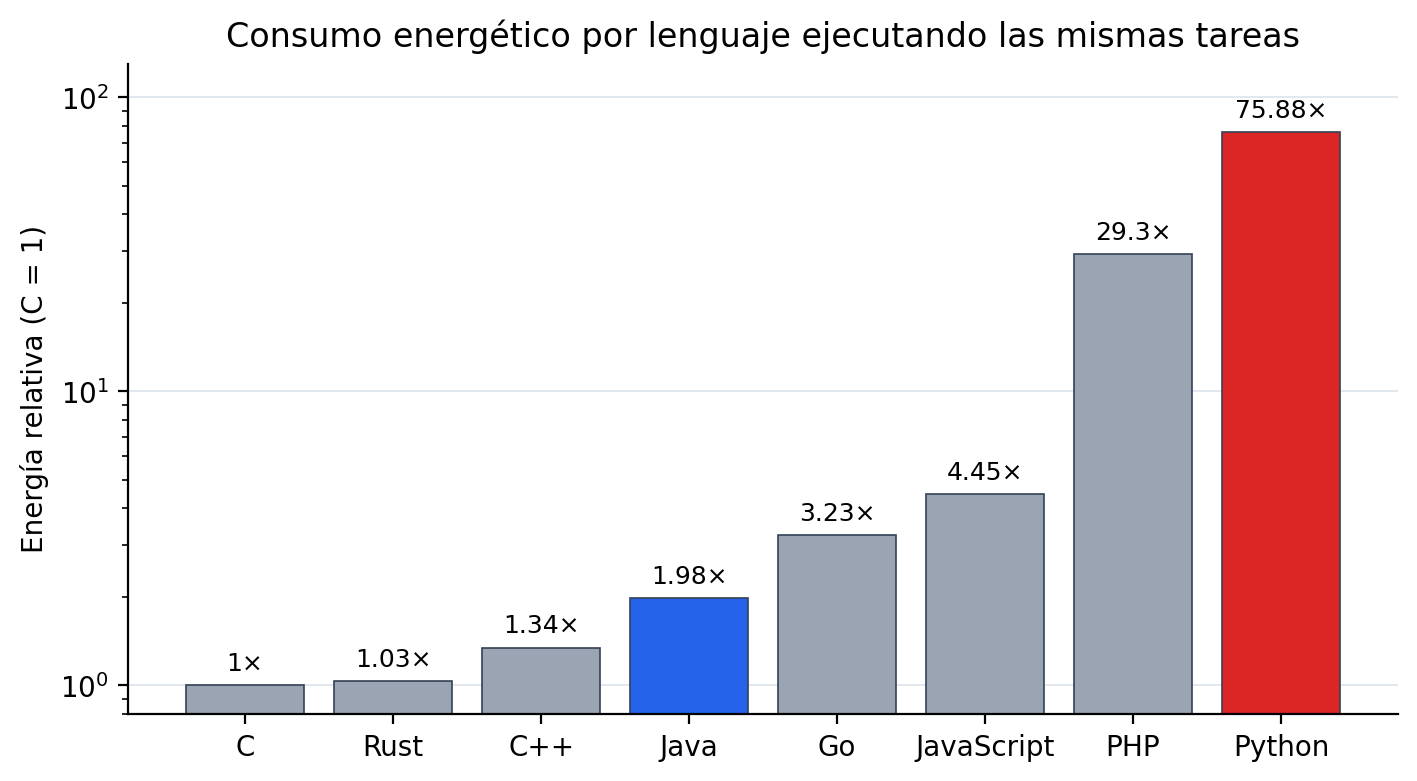
\includegraphics[width=0.9\textwidth]{consumo_lenguajes}
  \caption{Consumo energético relativo de varios lenguajes al ejecutar las
  mismas tareas, tomando C como referencia. Elaboración propia a partir de los
  datos de Pereira et al.~\cite{pereira2017}.}
  \label{fig:consumo-lenguajes}
\end{figure}


Sin embargo, el lenguaje elegido no es el único factor a tener en cuenta. Dentro de un mismo lenguaje, la manera de escribir el código también puede suponer una gran diferencia en el consumo. Por ejemplo, las estructuras de
datos elegidas, los algoritmos (como resolver un problema de forma recursiva o
iterativa) o los patrones de diseño influyen directamente en la energía que
acaba empleando el programa. De hecho, se ha demostrado que algunos de estos patrones pueden hacer que un programa consuma más o menos energía, dependiendo de cómo se implementen \cite{noureddine2025}. Por eso, optimizar el consumo de un software no depende de una sola decisión, sino de muchas que se toman a lo largo de todo el proceso de desarrollo. 

Ahora bien, para saber cuáles de estas decisiones son realmente mejores desde el punto de vista energético, primero es necesario medir cuánta energía consume un programa.

\subsection{Herramientas de medición existentes}
\label{subsec:herramientas-medicion}

Para medir el consumo energético existen numerosas herramientas, que pueden
clasificarse según el grado de detalle que ofrecen. Las más sencillas simplemente miden el consumo total de un equipo y muestran el valor real de la energía utilizada, mientras que
otras llegan a estimar el consumo de un programa concreto o incluso de cada una
de sus funciones, como es el caso de JoularJX. Estas últimas no pueden medirlo
directamente, ya que el hardware solo ofrece el consumo total, así que lo
calculan repartiendo esa energía en función del uso que cada proceso hace del procesador \cite{joularjx2022, joularjxrepo}. El problema es que, cuanto más baja una herramienta a este nivel de detalle, más útil resulta para mejorar el código, pero menos exactos son sus resultados, y de ahí la importancia de comprobar hasta qué punto son fiables.

Algunas solo
muestran el consumo total del sistema, como \texttt{perf} en Linux, que lee
directamente los contadores de energía del procesador (explicados en la
Sección~\ref{subsec:rapl}), pero otras, como PowerJoular \cite{joularjx2022}, Scaphandre
\cite{scaphandre} o PowerAPI \cite{fieni2024powerapi}, sí que distinguen cuánta energía gasta cada
programa en ejecución. Sin embargo, ninguna de
ellas permite saber qué partes específicas del código son las responsables de ese
gasto.

En el caso de Java, sí que existen algunas herramientas que llegan a medir el consumo de cada método por separado, aunque cuentan con una serie de limitaciones a tener en cuenta. jRAPL \cite{liu2015jrapl} es una librería que permite medir la energía de un fragmento de código, pero para ello obliga a modificar el propio programa, escribiendo a mano instrucciones que marquen dónde empieza y dónde acaba la parte que se quiere medir, y además lleva años sin actualizarse. Jalen \cite{noureddine2015hotspots}, desarrollada por el mismo autor que JoularJX, mide la energía de cada método sin que el programador tenga que tocar el código, pero para lograrlo modifica el programa por dentro de forma automática justo antes de ejecutarlo, lo que añade un consumo adicional, de manera que acaba alterando la propia medición \cite{noureddine2013review}, y por eso terminó abandonada en favor de JoularJX. Por último, JEPO \cite{kumar2019jepo} es un plugin para el IDE Eclipse, el cual surgió de un trabajo de investigación, que también mide por método, aunque insertando código de medición en cada uno de ellos, lo que lo hace poco ideal para programas con muchas líneas de código.


En la Tabla~\ref{tab:herramientas} que aparece a continuación, se resumen las principales características de
estas herramientas. JoularJX es la única que mide a nivel de método sin
necesidad de modificar el código y que, además, sigue en desarrollo activo y funciona en varios sistemas operativos.

\begin{table}[h]
	\centering
	\begin{tabular}{|l|l|l|l|}
		\hline
		\textbf{Herramienta} & \textbf{Nivel de detalle} & \textbf{Modifica el código} & \textbf{Estado} \\
		\hline
		perf & Sistema & No & Activa \\
		PowerJoular & Proceso & No & Activa \\
		Scaphandre & Proceso & No & Activa \\
		PowerAPI & Proceso & No & Activa \\
		jRAPL & Fragmento de código & Sí & Sin actualizar \\
		Jalen & Método & No & Abandonada \\
		JEPO & Método & Sí & Prototipo \\
		\textbf{JoularJX} & \textbf{Método} & \textbf{No} & \textbf{Activa} \\
		\hline
	\end{tabular}
	\caption{Comparativa de herramientas de medición del consumo energético.}
	\label{tab:herramientas}
\end{table}

\section{Técnicas y herramientas utilizadas}
\label{sec:tecnicas-utilizadas}

En esta sección se explica con más detalle cómo mide el procesador la energía
que gasta, cómo funciona JoularJX, qué son las librerías Jackson y Gson y qué
aporta JMH, con la que se preparan las pruebas.

\subsection{Medición de energía en el procesador}
\label{subsec:rapl}

Las herramientas que estiman el consumo de un programa necesitan saber cuánta energía utiliza el procesador. Los procesadores actuales de Intel y AMD miden esa energía mediante la interfaz RAPL (\emph{Running Average Power Limit}), que Intel introdujo en 2011 con su arquitectura Sandy Bridge y que AMD incorporó en 2017 en sus procesadores Ryzen. Aunque en un principio RAPL estaba pensada para limitar la potencia eléctrica del procesador, con el tiempo también empezó a usarse para medir el consumo de la CPU, ya que incluye unos contadores internos que llevan la cuenta de toda la energía que se va utilizando, de manera que se puede conocer cuánta energía se ha consumido en un intervalo de tiempo leyendo los valores del contador al principio y al final de dicho intervalo y restando ambos \cite{khan2018rapl}.


Además, el procesador se divide en varias zonas, llamadas dominios, cada una con su propio contador. Lo normal es que haya un dominio para el procesador entero, otro para los núcleos y, en algunos casos, otro para la memoria RAM, pero como no todos los procesadores son iguales, hay que comprobar cuáles están disponibles en el equipo que se vaya a utilizar, ya que en función de ellos los valores que se miden podrían ser diferentes.


En GNU/Linux, el sistema operativo da acceso a estos contadores a través del
subsistema \emph{powercap}, que los presenta como ficheros dentro de la carpeta
\texttt{/sys/class/powercap}. Cada dominio tiene su propio fichero
(\texttt{energy\_uj}) con la energía acumulada en microjulios, de forma que
cualquier programa puede leerlo como si fuera un fichero de texto normal. De
aquí es de donde JoularJX saca los datos de consumo en Linux. Eso sí, desde
2020 estos ficheros solo se pueden leer con permisos de administrador, porque
se descubrió que a partir de esos valores era posible deducir datos que el
equipo estaba procesando en ese momento, como claves de cifrado
\cite{lipp2021platypus}. Por eso, cualquier herramienta que quiera leerlos
necesita que antes se le dé permiso de lectura, algo que se detalla en el
Capítulo~\ref{cha:desarrollo}.


\subsection{JoularJX}
\label{subsec:joularjx}

JoularJX es una herramienta de código abierto, desarrollada por Adel Noureddine
en la Université de Pau et des Pays de l'Adour, que estima cuánta energía
consume cada método de un programa Java mientras se ejecuta
\cite{joularjx2022, joularjx3}. Para entender cómo lo consigue, primero hay que
ver cómo se ejecutan los programas escritos en Java.

\subsubsection{Funcionamiento como agente Java}
\label{subsubsec:agente-java}

A diferencia de otros lenguajes, un programa en Java no se ejecuta directamente
sobre el sistema operativo. El código se traduce primero a un formato
intermedio llamado \emph{bytecode}, y es la máquina virtual de Java
(\emph{Java Virtual Machine}, JVM) la que se encarga de ejecutarlo en cada
equipo. Gracias a esto, un mismo programa funciona igual en Windows, Linux o
macOS sin tener que cambiar nada.

Además, la JVM permite cargar agentes, que son pequeños programas que se
ejecutan dentro del mismo proceso que la aplicación y que pueden observar lo
que esta hace mientras está en marcha. Java ofrece para ello la API
\texttt{java.lang.instrument}, y basta con añadir la opción
\texttt{-javaagent} al arrancar el programa para que la JVM cargue el agente
junto a él. JoularJX funciona justo así, por lo que no hace falta modificar ni
recompilar el programa que se quiere medir, como se ve en el siguiente ejemplo.

\begin{verbatim}
java -javaagent:joularjx-3.1.0.jar -jar programa.jar
\end{verbatim}

\subsubsection{Obtención de la energía}
\label{subsubsec:obtencion-energia}

Una vez en marcha, lo primero que necesita JoularJX es saber cuánta energía
está gastando el procesador, y la forma de conseguirlo depende del sistema
operativo. En GNU/Linux lee directamente los contadores RAPL descritos en la
Sección~\ref{subsec:rapl}. Si el equipo ofrece un dominio que recoge el consumo
de toda la plataforma lo usa, y si no, suma el del procesador y el de la
memoria RAM. En Windows no se puede llegar a estos contadores directamente, así
que se apoya en un programa aparte del mismo proyecto, Power Monitor for
Windows \cite{winpowermonitor}. En macOS usa \texttt{powermetrics}, una
herramienta que ya viene con el sistema, y en dispositivos como la Raspberry
Pi, que no tienen este tipo de contadores, estima el consumo con modelos
calculados de antemano \cite{joularjx2022, joularjxrepo}.

\subsubsection{Reparto de la energía entre métodos}
\label{subsubsec:reparto-energia}

El problema es que el dato que llega del procesador corresponde a todo el
equipo, es decir, incluye también lo que gastan el resto de programas que haya
en marcha. Por eso JoularJX hace un reparto en tres pasos, que se repite cada
segundo y que se resume en la Figura~\ref{fig:esquema-joularjx}.

En primer lugar, calcula qué parte de esa energía corresponde al programa que
se está midiendo. Para ello compara el uso de CPU del proceso de la JVM con el
uso de CPU total del sistema y le asigna la misma proporción de energía. Por
ejemplo, si en un segundo el procesador ha consumido 20 julios y el programa ha
supuesto la mitad de todo el uso de CPU, se le atribuyen 10 julios.

En segundo lugar, reparte esa energía entre los hilos del programa según el
tiempo de CPU que ha usado cada uno, ya que un programa Java suele tener varios
hilos trabajando a la vez.

Por último, tiene que averiguar qué método se estaba ejecutando en cada hilo.
Para ello, cada 10 milisegundos consulta la pila de llamadas de todos los
hilos, que es la lista de métodos que están en ejecución en ese momento y desde
dónde se ha llamado a cada uno, y apunta cuál es el que se está ejecutando en
ese instante. Al cabo de un segundo tiene unas cien muestras por hilo, y la
energía de cada hilo se reparte entre sus métodos según las veces que ha
aparecido cada uno. Si un método aparece en el 30\% de las muestras, se le
asigna el 30\% de la energía de ese hilo \cite{joularjx2022, joularjx3}.

Esta técnica se conoce como muestreo, y su ventaja es que JoularJX se limita a
observar el programa desde fuera, sin añadir instrucciones dentro de cada
método como hacían Jalen o JEPO. A cambio, el resultado es una estimación y no
una medida exacta.

\begin{figure}[h]
  \centering
  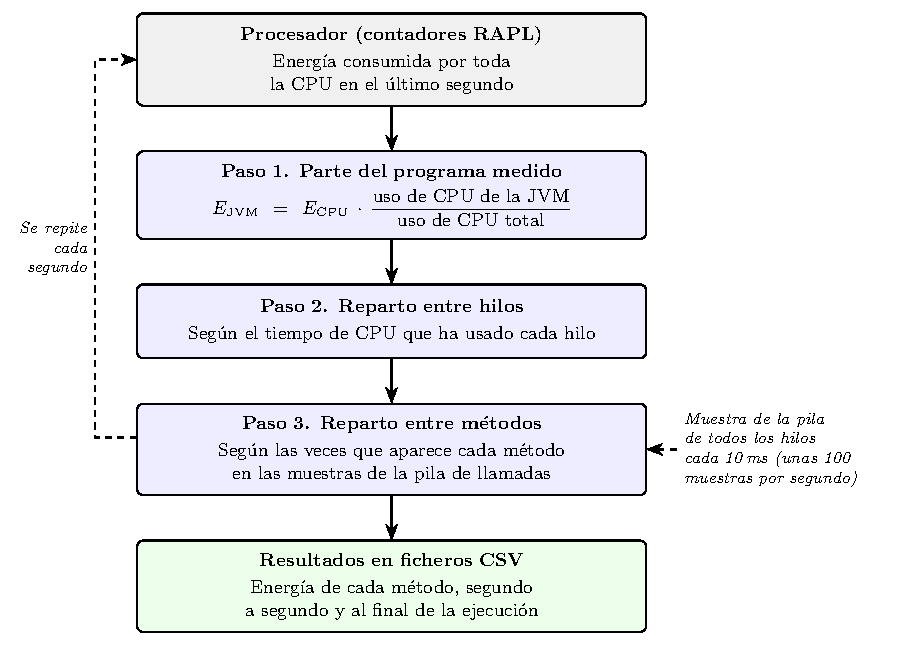
\includegraphics[width=0.9\textwidth]{esquema_joularjx}
  \caption{Proceso que sigue JoularJX cada segundo para repartir la energía del
  procesador entre los métodos de un programa.}
  \label{fig:esquema-joularjx}
\end{figure}

\subsubsection{Configuración y resultados}
\label{subsubsec:config-resultados}

El comportamiento de JoularJX se controla mediante un fichero llamado
\texttt{config.\allowbreak properties}, que tiene que estar en la carpeta desde la que se
lanza el programa o indicarse su ruta al arrancarlo. Entre otras cosas, permite
cambiar cada cuánto se toman las muestras de la pila (entre 1 y 1000
milisegundos), ocultar el consumo de los propios hilos del agente o indicar qué
partes del programa interesa analizar mediante la opción
\texttt{filter-\allowbreak method-\allowbreak names} \cite{joularjxrepo}.

Los resultados se guardan en ficheros CSV dentro de una carpeta llamada
\texttt{joularjx-results}, separados en dos grupos. Por un lado están los datos
de todos los métodos, incluidos los de las propias librerías de Java, y por
otro, solo los de los métodos filtrados. En este segundo grupo, la energía que
gastan las funciones de Java a las que llama un método se le suma a ese método.
Por ejemplo, si un método del programa llama a \texttt{println} para escribir
un texto en pantalla, el consumo de \texttt{println} se cuenta como parte del
método que la ha llamado. Esto es muy útil en este trabajo, porque permite ver
cuánto gastan los métodos de Jackson y Gson incluyendo todo el trabajo que
delegan en otras partes de Java. Para cada grupo se generan ficheros con el
consumo segundo a segundo, con el total al terminar el programa y con la
evolución de cada método a lo largo del tiempo.

\subsubsection{Limitaciones}
\label{subsubsec:limitaciones-joularjx}

Hay que tener en cuenta que todo este proceso da una estimación. El reparto
supone que el uso de CPU refleja bien el consumo real, y el muestreo puede
pasar por alto métodos muy rápidos que se ejecuten entre dos muestras. Además,
la energía de partida es la que mide RAPL, que no incluye otros componentes del
equipo como el disco.

Brunnert \cite{brunnert2025accuracy} comparó la energía que JoularJX atribuye a
una aplicación Java con la que mide RAPL para todo el sistema, con distintos
niveles de carga, y comprobó que ambas coinciden casi por completo, con
diferencias de entre el 0,4\% y el 2,8\%. Las diferencias eran mayores cuanto
menor era la carga, porque entonces pesa más lo que consume el resto del
sistema. Sin embargo, este estudio se centra en el consumo del programa
completo y no comprueba si el reparto entre métodos es correcto, que es
precisamente lo más difícil de verificar. Comprobar hasta qué punto estas
limitaciones afectan a los resultados es uno de los objetivos de este trabajo
(Sección~\ref{sec:objetivos}).


\subsection{JSON, Jackson y Gson}
\label{subsec:json-jackson-gson}

% QUÉ PONER:
% - Qué es JSON y para qué se usa (intercambio de datos entre aplicaciones,
%   APIs web).
% - Qué es serializar y deserializar.
% - Jackson: quién la desarrolla y cómo funciona por dentro (cita jackson).
% - Gson: quién la desarrolla y cómo funciona por dentro (cita gson).
% - En qué se diferencian, que es lo que justifica compararlas.


\subsection{JMH}
\label{subsec:jmh}

% QUÉ PONER:
% - Qué es JMH (Java Microbenchmark Harness) y quién lo desarrolla.
% - Por qué hace falta: el calentamiento de la JVM (compilación JIT) hace
%   que medir "a mano" dé resultados poco fiables.
% - Qué aporta: iteraciones de calentamiento, repeticiones y resultados
%   estadísticos.
% (Cita pendiente de añadir al .bib.)


%%% Local Variables:
%%% TeX-master: "../book"
%%% End:
